\documentclass[11pt,compress,t,notes=noshow, aspectratio=169, xcolor=table]{beamer}

\usepackage[]{../../style/lmu-lecture}
% Defines macros and environments
\input{../../style/common.tex}


\title{Applied Machine Learning}
% \author{LMU}
%\institute{\href{https://compstat-lmu.github.io/lecture_iml/}{compstat-lmu.github.io/lecture\_iml}}
\date{}

\begin{document}

\newcommand{\titlefigure}{figure/empty}
\newcommand{\learninggoals}{
	%\item Imputation
    \item Feature Filtering
    \item Feature Selection}

\lecturechapter{Feature Engineering}
\lecture{Applied Machine Learning}

\section{Recap}

\begin{frame}{What is feature engineering?}
\begin{itemize}
    \item 
\end{itemize}
\end{frame}

\begin{frame}{Train-Test Leakage}
% This is so important, that I will just repeat this again!
\begin{itemize}
    \item 
\end{itemize}
\end{frame}

\begin{frame}{Types of Feature Engineering (so far)}
\begin{itemize}
    \item numerical encoding of categorical features
    \item feature transformations
    \item imputation
\end{itemize}
\end{frame}

\section{Feature Selection}

\begin{frame}{}
\includepdf[pages={3},trim=0 20 0 0,clip,width=490pt,offset=-10pt 10pt,pagecommand={}]{sl/slides-fs-introduction.pdf}
\end{frame}

\begin{frame}{}
\includepdf[pages={4},trim=0 20 0 0,clip,width=490pt,offset=-10pt 10pt,pagecommand={}]{sl/slides-fs-introduction.pdf}
\end{frame}

\begin{frame}{}
\includepdf[pages={5},trim=0 20 0 0,clip,width=490pt,offset=-10pt 10pt,pagecommand={}]{sl/slides-fs-introduction.pdf}
\end{frame}

\begin{frame}{}
\includepdf[pages={6},trim=0 20 0 0,clip,width=490pt,offset=-10pt 10pt,pagecommand={}]{sl/slides-fs-introduction.pdf}
\end{frame}

\begin{frame}{Reasons for feature selection}
\begin{itemize}
    % All from https://mlr3book.mlr-org.com/chapters/chapter6/feature_selection.html#sec-fs-filter
    \item improved predictive performance, since we reduce overfitting on irrelevant features,
    \item robust models that do not rely on noisy features,
    \item simpler models that are easier to interpret,
    \item faster model fitting, e.g. for model updates,
    \item faster prediction, and
    \item no need to collect potentially expensive features.
\end{itemize}
\end{frame}

\begin{frame}{Goals of feature selection}
% Source: https://link.springer.com/article/10.1007/s10618-020-00731-7
\vfill
\textbf{Single feature selection problem:} identifying a minimal-size subset of the variables that is optimally predictive for an outcome variable T of interest.

%\vspace{1cm}
\vfill

% For this lecture the multiple feature selection problem is not relevant, but it is important that you have heard about it
\textbf{Multiple Feature Selection Problem:} Let $\mathcal{S}$ be the solution to the single feature selection problem (called the reference solution). The solution $\mathcal{M}$ to the multiple feature selection problem consists of all minimal-size sets $\mathcal{S}_i \in \mathcal{F}$  that are statistically equivalent to $\mathcal{S}$.
\begin{itemize}
    \item Important for knowledge discovery (know all possible solutions)
    \item We will not delve into this any further
\end{itemize}
\vfill
\end{frame}

\begin{frame}{}
\includepdf[pages={8},trim=0 20 0 0,clip,width=490pt,offset=-10pt 10pt,pagecommand={}]{sl/slides-fs-introduction.pdf}
\end{frame}

\section{Filtering}

\begin{frame}{}
\includepdf[pages={2},trim=0 20 0 0,clip,width=490pt,offset=-10pt 10pt,pagecommand={}]{sl/slides-fs-filters1.pdf} 
\end{frame}

\begin{frame}{}
\includepdf[pages={4},trim=0 20 0 0,clip,width=490pt,offset=-10pt 10pt,pagecommand={}]{sl/slides-fs-filters1.pdf} 
\end{frame}

\begin{frame}{}
\includepdf[pages={5},trim=0 20 0 0,clip,width=490pt,offset=-10pt 10pt,pagecommand={}]{sl/slides-fs-filters1.pdf} 
\end{frame}

\begin{frame}{}
\includepdf[pages={7},trim=0 20 0 0,clip,width=490pt,offset=-10pt 10pt,pagecommand={}]{sl/slides-fs-filters1.pdf} 
\end{frame}

\begin{frame}{Further Criteria/Methods}
    \begin{itemize}
        \item Classification
        \begin{itemize}
            \item $\chi^2$-statistic
            \item Welch's t-Test
            \item F-Test
            
        \end{itemize}
        \item Regression \& Classification
        \begin{itemize}
            \item Mutual Information
            \item Relief
        \end{itemize}
        \item Model-based
        \begin{itemize}
            \item Tree-based feature importance (decision tree, extra trees, random forest)
            \item Coefficients of linear model
        \end{itemize}
    \end{itemize}
\end{frame}

\begin{frame}{}
\includepdf[pages={5},trim=0 20 0 0,clip,width=490pt,offset=0pt 10pt,pagecommand={}]{sl/slides-fs-filters2.pdf} 
\end{frame}

\begin{frame}{Advantages and Disadvantages}
    Advantages
    \begin{itemize}
        \item Fast
        \item Typically scales well with the number of features $p$
        \item Generally interpretable
        \item Can be used with any inducer
    \end{itemize}
    Negative
    \begin{itemize}
        \item Does not take specifics of the inducing algorithm into account
        \item Redundant features will have similar weights
        \item Often univariate
    \end{itemize}
\end{frame}

\section{Wrapper}

\begin{frame}{}
\includepdf[pages={2},trim=0 20 0 0,clip,width=490pt,offset=0pt 10pt,pagecommand={}]{sl/slides-fs-wrapper.pdf} 
\end{frame}

\begin{frame}{}
\includepdf[pages={3},trim=0 20 0 0,clip,width=490pt,offset=0pt 10pt,pagecommand={}]{sl/slides-fs-wrapper.pdf} 
\end{frame}

\begin{frame}{}
\includepdf[pages={4},trim=0 20 0 0,clip,width=490pt,offset=0pt 10pt,pagecommand={}]{sl/slides-fs-wrapper.pdf} 
\end{frame}

\begin{frame}{}
\includepdf[pages={5},trim=0 20 0 0,clip,width=490pt,offset=0pt 10pt,pagecommand={}]{sl/slides-fs-wrapper.pdf} 
\end{frame}

\begin{frame}{}
\includepdf[pages={6},trim=0 20 0 0,clip,width=490pt,offset=0pt 10pt,pagecommand={}]{sl/slides-fs-wrapper.pdf} 
\end{frame}

\begin{frame}{}
\includepdf[pages={7},trim=0 20 0 0,clip,width=490pt,offset=0pt 10pt,pagecommand={}]{sl/slides-fs-wrapper.pdf} 
\end{frame}

\begin{frame}{}
\includepdf[pages={8},trim=0 20 0 0,clip,width=490pt,offset=0pt 10pt,pagecommand={}]{sl/slides-fs-wrapper.pdf} 
\end{frame}

\begin{frame}{}
\includepdf[pages={9},trim=0 20 0 0,clip,width=490pt,offset=0pt 10pt,pagecommand={}]{sl/slides-fs-wrapper.pdf} 
\end{frame}

\begin{frame}{Advantages and Disadvantages}
    Advantages
    \begin{itemize}
        \item Inducer-agnostic
        \item Any performance measure can be used
        \item Optimizes the desired performance measure directly
    \end{itemize}
    Disadvantages
    \begin{itemize}
        \item Expensive
        \item Does not scale well with the number of features
        \item Does (in general) not use additional info about model structure
        \item Nested resampling becomes necessary
    \end{itemize}
    
\end{frame}

\section{Embedded}

\begin{frame}{Regularization}
    
\end{frame}

% Overview: https://www.frontiersin.org/articles/10.3389/fbinf.2022.927312/full#h3
\begin{frame}{Tree methods}
    
\end{frame}

\section{Features to drop}
% ID columns, identical columns
\begin{frame}{Features to Drop}
\begin{itemize}
    \item ID columns
    \begin{itemize}
        \item Often ordered, can leak time information
        \item Contains no information that can generalize
    \end{itemize}
    \item Duplicate features
    \begin{itemize}
        \item Cause issues for (linear) models
        \item Slow down learning
        \item Reduce model interpretability
    \end{itemize}
\end{itemize}
\end{frame}

\section{Multi-objective optimization of features}

\begin{frame}{Challenge(s)}
    \begin{itemize}
        \item Two competing objectives:
        \begin{enumerate}
            \item goodness-of-fit
            \item number of variable
        \end{enumerate}
    \end{itemize}
\end{frame}

\section{Wrap-up}

\endlecture
\end{document}
